\documentclass[10pt,twocolumn,letterpaper]{article}

\usepackage{cvpr}
\usepackage{times}
\usepackage{epsfig}
\usepackage{graphicx}
\usepackage{amsmath}
\usepackage{amssymb}
\usepackage{enumitem}
\usepackage{subcaption}

% Include other packages here, before hyperref.

% If you comment hyperref and then uncomment it, you should delete
% egpaper.aux before re-running latex.  (Or just hit 'q' on the first latex
% run, let it finish, and you should be clear).
\usepackage[breaklinks=true,bookmarks=false]{hyperref}

\cvprfinalcopy % *** Uncomment this line for the final submission

\def\cvprPaperID{****} % *** Enter the CVPR Paper ID here
\def\httilde{\mbox{\tt\raisebox{-.5ex}{\symbol{126}}}}

% Pages are numbered in submission mode, and unnumbered in camera-ready
%\ifcvprfinal\pagestyle{empty}\fi
\setcounter{page}{1}
\begin{document}

%%%%%%%%% TITLE
\title{Deep Dish : Deep Learning for Classifying Food Dishes}

\author{Abhishek Goswami\\
Microsoft\\
Redmond, WA\\
{\tt\small agoswami@microsoft.com}
% For a paper whose authors are all at the same institution,
% omit the following lines up until the closing ``}''.
% Additional authors and addresses can be added with ``\and'',
% just like the second author.
% To save space, use either the email address or home page, not both
\and
Haichen Liu\\
Dropbox\\
Seattle, WA\\
{\tt\small haichen@dropbox.com}
}

\maketitle
%\thispagestyle{empty}

%%%%%%%%% ABSTRACT
\begin{abstract}
   %The ABSTRACT is to be in fully-justified italicized text, at the top
   %of the left-hand column, below the author and affiliation
   %information. Use the word ``Abstract'' as the title, in 12-point
   %Times, boldface type, centered relative to the column, initially
   %capitalized. The abstract is to be in 10-point, single-spaced type.
   %Leave two blank lines after the Abstract, then begin the main text.
   %Look at previous CVPR abstracts to get a feel for style and length.
	
	We consider the problem of classifying food dishes. Food items have unique characteristics - they come in different colors and shapes, can be clustered into groups (e.g. fruits, vegetables), and can be combined in several ways to prepare a meal etc. This makes images of food dishes particularly interesting to classify. We show that convolutional neural networks are quite suitable for this task, and outperform traditional machine learning approaches in classifying food dishes.
		
\end{abstract}

%%%%%%%%% BODY TEXT
\section{Introduction}


This project aims to use deep learning on images of food dishes. Food images are unique: there are multiple cuisines around the world; food items have unique color, size, shape and texture; and food items can be combined in several ways to prepare a meal. Using artificial intelligence on food images has the potential to revolutionize the field of dining, promote healthy eating, prevent food waste etc.

To that end, we are working on the problem of classifying food dishes. We formulate this problem as a classification task with one class per image, i.e given an image of a food dish, we want to correctly predict what dish it is. Figure~\ref{fig:imgsburgerpizza} shows sample images of two popular food categories. Being able to accurately predict a food category from an image could be useful for several application scenarios, such as knowing the calorie count for that food item, identifying its ingredients etc.  

The remainder of the paper is organized as follows. In Section~\ref{sec:relatedwork} we survey related work in the area of image classification. In Section~\ref{sec:methods} we introduce the key components used in image classification tasks. In Section~\ref{sec:datasetandfeatures} we provide details about our dataset. Section~\ref{sec:evaluationresults}  presents the experimental results from our modeling techniques. Finally, we present our conclusions in Section~\ref{sec:conclusion}.

\begin{figure}[ht!]
    \centering
    \begin{subfigure}{.4\linewidth}
        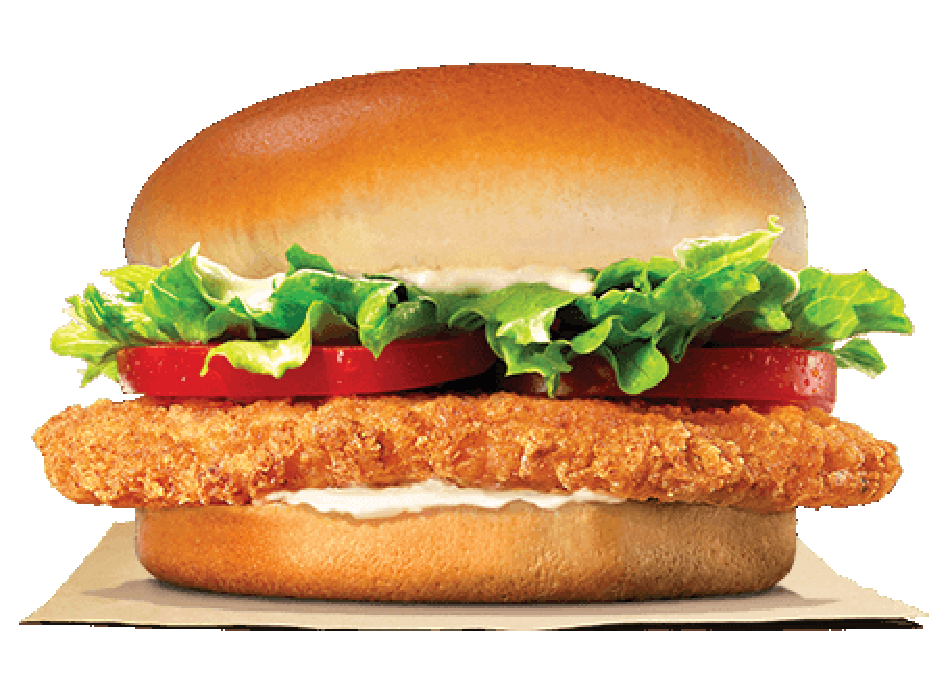
\includegraphics[height=1.25in, width=1.6in]{Figs4Paper/_final/img_burger.eps}
        \caption{burger}
    \end{subfigure}
    \hskip2em
    \begin{subfigure}{.4\linewidth}
        
\includegraphics[height=1.25in, width=1.6in]{Figs4Paper/_final/img_pizza.eps}
        \caption{pizza}
    \end{subfigure}
    \caption{Sample images in our dataset}
		\label{fig:imgsburgerpizza}
\end{figure}

%-------------------------------------------------------------------------

\section{Related Work}
\label{sec:relatedwork}

%You should find existing papers, group them into categories based on their approaches, and talk about them: Discuss strengths and weaknesses. In your opinion, which approaches were clever/good? What is the state-of-the-art? Do most people perform the task by hand?
%
%You should have at least 15 references in the related work. Include previous attempts by others at your problem, previous technical methods, or previous learning algorithms. Google Scholar is very useful for this: https://scholar.google.com/ (you can click “cite” and it generates MLA, APA, BibTeX, etc.) You can also try http://www.arxiv-sanity.com/ to search for recent arXiv papers. Try to cite academic publications only (i.e., try to avoid citing blog posts or news articles). Note: arXiv citations are acceptable.

%-------------------------------------------------------------------------

Deep Convolutional Neural Networks have been shown to be very useful for visual recognition tasks. AlexNet~\cite{krizhevsky2012imagenet} won the ImageNet Large Scale Visual Recognition Challenge~\cite{russakovsky2015imagenet} in 2012, spurring a lot of interest in using deep learning to solve challenging problems. Since then, deep learning has been used successfully in multiple fields like machine vision, facial recognition, voice recognition, natural language processing etc.

There are several flavors of image classification tasks that have been been proposed over the years. These range from being able to recognize hadwritten digits~\cite{lecun1990handwritten} to classifying plants using the images of leaves~\cite{kaggleleaf}.   

Our problem of classifying food dishes is unique. We did not find any existing work focussed on classifying food dishes from images. The closest example of a food-related task we could find was a \textit{restaurant classification} problem from Yelp~\cite{kagglerestaurantyelp}. In their scenario, they want to classify the images of \textit{restaurants} along some business attributes (e.g restaurant is kid friendly, has table service  etc). Classifying food dishes from images presents several distinct characteristics that we discuss in Sections~\ref{sec:datasetandfeatures} and~\ref{sec:evaluationresults}







\section{Methods}
\label{sec:methods}

Image classification is the task of assigning a single label to an image (or rather an array of pixels that represents an image) from a fixed set of categories. A complete pipeline for this task is as follows:
\begin{itemize}[noitemsep]
\item \textbf{Input} : A set of $N$ images, each labeled with one of $K$ different classes. This data is referred to as the \textit{training set}.
\item \textbf{Learning} (aka Training) : Use the \textit{training set} to learn the characteristics of each class. The output of this step is a \textit{model} which will be used for making predicions.
\item \textbf{Evaluation}  : Evaluate the quality of the \textit{model} by asking it to make predictions on a new set of images that it has not seen before (also referred to as the \textit{test set}). This evaluation is done by comparing the true labels (aka ground truth) of the \textit{test set} with the predicted labels output by the learned \textit{model}.
\end{itemize}

The formal approach for solving the problem of image classification can be broken down into several key components which we discuss next.

\subsection{Score Function}
\label{subsec:scorefunction}

The score function maps the raw data to class scores. For a linear classifier, the score function can be defined as: 
\begin{align}
f(\boldsymbol{x_{i}}, \boldsymbol{W}, \boldsymbol{b}) = \boldsymbol{W} \boldsymbol{x_{i}} + \boldsymbol{b}.\label{eqn:scorefunction}
\end{align}

where $\boldsymbol{x_{i}}$ represents the input image. The matrix $\boldsymbol{W}$, and the vector $\boldsymbol{b}$ are the parameters of the function, and represent the weights and bias respectively.

In image classification, the score function takes an image ${\boldsymbol {x_{i}}}$ and computes the vector $f(\boldsymbol{x_{i}}, \boldsymbol{W})$ of the raw class scores (which we abbreviate as ${\boldsymbol {s}}$). So, given an image ${\boldsymbol {x_{i}}}$, the predicted score for the j-th class is the j-th element in $\boldsymbol{s}$ : $\boldsymbol{s}_{j} = f(\boldsymbol{x_{i}}, \boldsymbol{W})_{j}$. We use the  class scores from our training data to compute the loss.

\subsection{Loss Function}
\label{subsec:lossfunction}

The loss function quantifies the match between the predicted \textit{scores} and the ground truth labels in the training data. The loss function (also referred to as the cost function or objective) can be viewed as the unhappiness of the predicted scores output by the score function. Intuitively, the loss would be low if the predicted scores match the training data labels closely. Otherwise the loss would be high. Next, we discuss the two common classifiers with details about their respective loss functions. 

\subsection{Classifiers}
\label{subsec:classifiers}

In this section we discuss two common classifiers that are often used in image classification tasks: the \textbf{SVM Classifier} and the \textbf{Softmax Classifier}. For both of them the function mapping the input image $\boldsymbol{x_{i}}$ to the raw class scores $\boldsymbol{s} = f(\boldsymbol{x_{i}}, \boldsymbol{W})$ remains the same. But the Softmax classifier has one additional step : it uses the softmax function to squash the raw scores in $\boldsymbol{s}$ into a vector of values between zero and one, that sum to one.  We discuss the details of each classifier below.

\subsubsection{SVM Classifier}
\label{subsubsec:svmclassifier}

The SVM classifier uses the \textit{hinge loss} (also referred to as \textit{max-margin loss}, or \textit{SVM loss}). For the i-th example in our data, the \textit{hinge loss} is given as:

\begin{align}
L_{i} = \sum_{j \neq y_{i}} \max(0, \boldsymbol{s}_{j} - \boldsymbol{s}_{y_{i}} + \Delta).\label{eqn:svmloss}
\end{align}

where $\Delta$ is a hyperparameter which represents that the SVM loss function in equation~\ref{eqn:svmloss} wants the score of the correct class $\boldsymbol{y_{i}}$ to be larger than the incorrect class scores by at least $\Delta$. Otherwise we incur loss. 

\subsubsection{Softmax Classifier}
\label{subsubsec:softmaxclassifier}

The Softmax classifier uses the \textit{cross entropy loss} (also referred to as \textit{softmax loss}). For the i-th example in our data, the \textit{cross entropy loss} is given as:

\begin{align}
L_{i} =  - \log \frac {e^{f_{y_i}}} {\sum_{j} e^{f_{j}}}.\label{eqn:softmaxloss}
\end{align}

where $f_{j}$ means the j-th element of the vector of class scores $f$. Note that the softmax classifier uses the softmax function to squash the raw class scores ${\boldsymbol {s}}$ into normalized positive values that sum to one, so that the cross entropy loss can be applied. The \textbf{softmax function} can be represented as:

\begin{align}
f_{j} (z) =  \frac {e^{z_j}} {\sum_{k} e^{z_{k}}}.\label{eqn:softmaxfunction}
\end{align}

It takes a vector of real-valued scores (in z) and squashes it to a vector of values between zero and one, that sum to one.

\subsection{Total Loss}
\label{subsec:totalloss}

For both the SVM Classifier and the Softmax Classifier, the full loss for the dataset is the mean of $L_{i}$ over all training examples, together with a regularization term, $R(W)$

\begin{align}
L =  \frac {\sum_{i} L_{i}} {N} +  \lambda R(W).\label{eqn:totalloss}
\end{align}

where $N$ represents the total number of images in the training set. $\lambda$ is a hyperparameter, often referred to as \textit{regularization strength}. The loss function lets us quantify the quality of any particular set of parameters in our model, the lower the loss the better. We next discuss strategies of how to minimize the loss.

\subsection{Optimization}
\label{subsec:optimization}

Optimization is the process of finding the set of parameters of our model that minimize the total loss, defined in equation~\ref{eqn:totalloss}

The core principle behind optimization techniques is to compute the \textbf{gradient} of the loss with respect to the parameters of the model. The gradient of a function gives the direction of steepest ascent. One way of computing the gradient efficiently is to compute the gradient analytically using a recursive application of the \textbf{chain rule}. This technique is called \textbf{backpropagation}~\cite{lecun2012efficient} and it allows us to efficiently optimize arbitrary loss functions. These loss functions  may be expressing different kinds of network architectures (e.g. fully connected neural networks, convolutional networks etc). Backpropagation is our tool of choice for computing the gradients in all such cases.  

\subsubsection{Parameter Updates}
\label{subsubsec:parameterupdates}
   
Once the analytic gradient is computed using backpropagation, the gradients are used to perform a parameter update. There are several approaches for performing the update that have been proposed in literature: SGD~\cite{bottou2010large}, SGD+Momentum~\cite{qian1999momentum, sutskever2013importance}, Nesterov Momentum~\cite{nesterov1983method}, Adagrad~\cite{duchi2011adaptive}, RMSprop~\cite{hinton2012neural}, Adam~\cite{kingma2014adam} etc.

%-------------------------------------------------------------------------
\section{Dataset and Features}
\label{sec:datasetandfeatures}

We start with a discussion about our data collection methodology. We then present details about the data pre-processing steps. Finally we round up this section with details about our dataset.

We provide some details about our dataset below.

\subsection{Data Collection}
\label{subsec:datacollection}

We collected our dataset using the Google Image Search~\cite{googleimagesearch} and the Bing Image Search API~\cite{bingimagesearchapi}. We also explored the use of ImageNet~\cite{imagenet} and Flickr~\cite{flickr} for collecting images. However, we found the images from Google and Bing to be much more representative of the classes they belonged to, compared to the images from ImageNet and Flickr. ImageNet and Flickr seem to have a lot of spurious images (images which clearly do not belong to the class). Hence we decided to use the images we could collect from Google and Bing.

\subsection{Pre-Processing Steps}
\label{subsec:preprocessingsteps}

We re-sized all of our images to have height, width and channel dimensions of 32, 32 and 3 respectively. This was done primarily for computational efficiency in performing our experiments. We filtered out images which we were unable to resize to our specified height, width and channel requirements. Unfortunately, this meant losing approx ~10\% of the data from our original dataset. Figure~\ref{fig:imgsburgerpizza} shows a two sample images from our dataset. As a part of pre-processing, we also subtract the mean image from all the images in our dataset. The mean image is computed using the image mean of the training data

\subsection{Dataset Details}

\begin{table}
\begin{center}
\begin{tabular}{|l|c|}
\hline
Dataset & Num of Images \\
\hline
Train & 18,927 \\
Validate & 5,375 \\
Test & 2,682 \\
\hline
\end{tabular}
\end{center}
\caption{Dataset split for train, validation and test sets.}
\label{table:datasplitdetails}
\end{table}

After the pre-processing steps described in Section~\ref{subsec:preprocessingsteps} we had a total of 26,984 images. We then split our dataset randomly into 3 disjoint sets: Train(70\% approx.), Validate(20\% approx.) and Test(10\% approx.). Table~\ref{table:datasplitdetails} provides a count of the number of images in each set.

Currently our dataset has 20 classes.  This corresponds to 20 popular food dishes from around the world. Table~\ref{table:classdistribution} shows the class label distribution of the dataset. The distribution of the number of images in each class is mostly uniform. 

\begin{table}
\begin{center}
\begin{tabular}{|l|c|}
\hline
Food Item & Number of Images \\
\hline\hline
dumplings & 1,091\\
dal & 1,031\\
ramen & 1,023\\
icecream & 1,021\\
naan & 1,020\\
sushi & 1,020\\
cordonbleu & 1,018\\
pasta & 1,002\\
lasagna & 971\\
friedrice & 966\\
roastturkey & 930\\
padthai & 919\\
burger & 912\\
samosa & 897\\
burrito & 888\\
pizza & 885\\
bratwurst & 876\\
biryani & 865\\
sandwich & 847\\
fries & 745\\
\hline
\end{tabular}
\end{center}
\caption{Class distribution}
\label{table:classdistribution}
\end{table}


%-------------------------------------------------------------------------
\section{Evaluation Results}
\label{sec:evaluationresults}

In this section we discuss our experiments and results. We chose accuracy as our evaluation metric when comparing different models. For brevity, we are reporting the accuracy numbers to two decimal places. 

For Section~\ref{subsec:linearclassifiersonrawimagepixels}, Section~\ref{subsec:neuralnetworksonrawimagepixels} and Section~\ref{subsec:imagefeatures} we re-purposed code from assignments 1 and 2 in Stanford University's Spring 2017 course, CS231N: Convolutional Neural Networks for Visual Recognition~\cite{cs231n}. For Section~\ref{subsec:convolutionalnetworks} and Section~\ref{subsec:transferlearning}, we use TensorFlow~\cite{abadi2016tensorflow} for training our convolutional network models.

\begin{table*}[h!]
\begin{center}
\begin{tabular}{|l|c|c|}
\hline
Modeling Approach & Best Validation Accuracy & Test Set Accuracy \\
\hline\hline
Linear SVM on raw image pixels & 0.18 & 0.16 \\
Five layer fully connected neural net on raw image pixels & 0.19 & 0.18 \\
Linear SVM on image features & 0.21 & 0.22 \\
Two layer neural net on image features & 0.26 & 0.27 \\
Training a Convolutional Network from scratch  & 0.40 & 0.40 \\
Transfer Learning (by fine tuning a VGG model) & 0.46 & 0.45 \\
\hline
\end{tabular}
\end{center}
\caption{Summary of results across different modeling approaches.}
\label{table:accuracyresults}
\end{table*}

\subsection{Linear classifiers on raw image pixels}
\label{subsec:linearclassifiersonrawimagepixels}

%\begin{figure} 
%\centering
%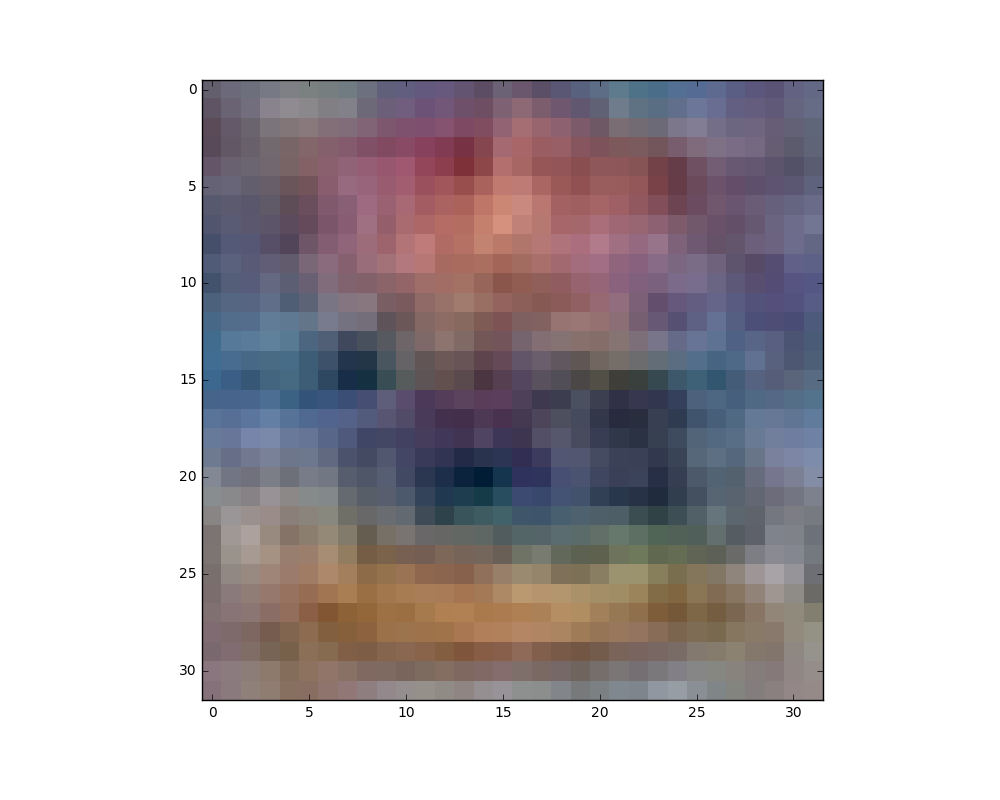
\epsfig{file=Figs4Paper/_final/svm_learnedweights_burger.eps, height=1.25in, width=1.6in} 
%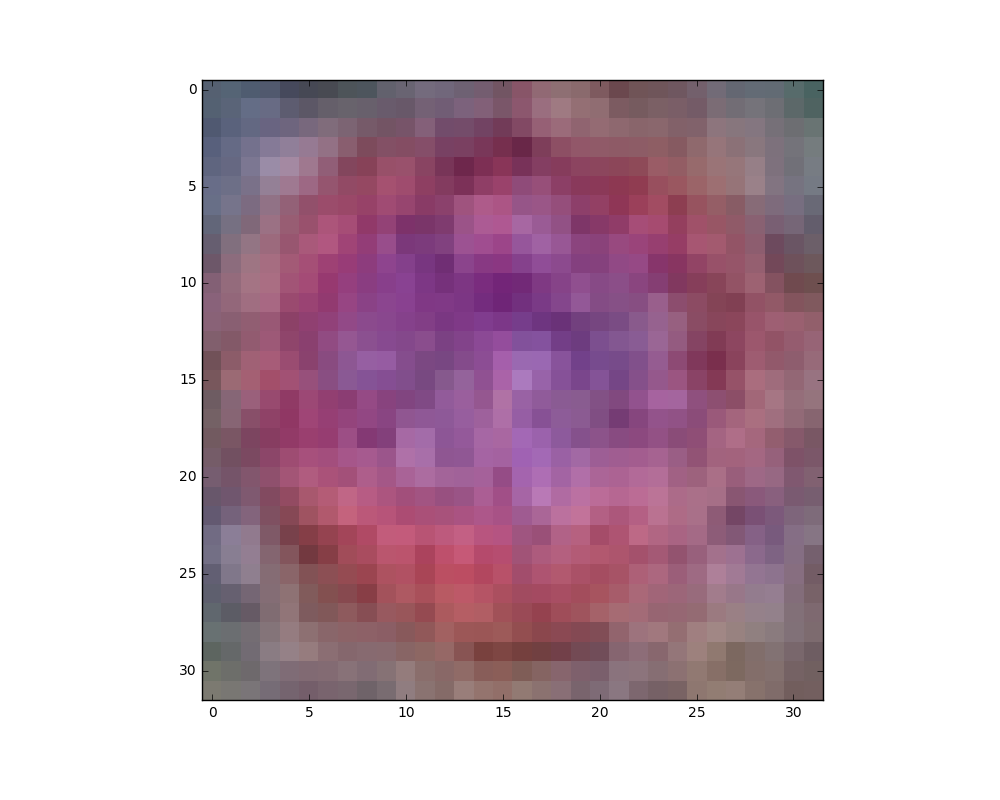
\epsfig{file=Figs4Paper/_final/svm_learnedweights_pizza.eps, height=1.25in, width=1.6in}
%\caption{Visualizing the weights learned by the SVM model for the burger and pizza classes}
%\label{fig:learnedweightsburgerpizza}
%\end{figure}

\begin{figure}[ht!]
    \centering
    \begin{subfigure}{.4\linewidth}
        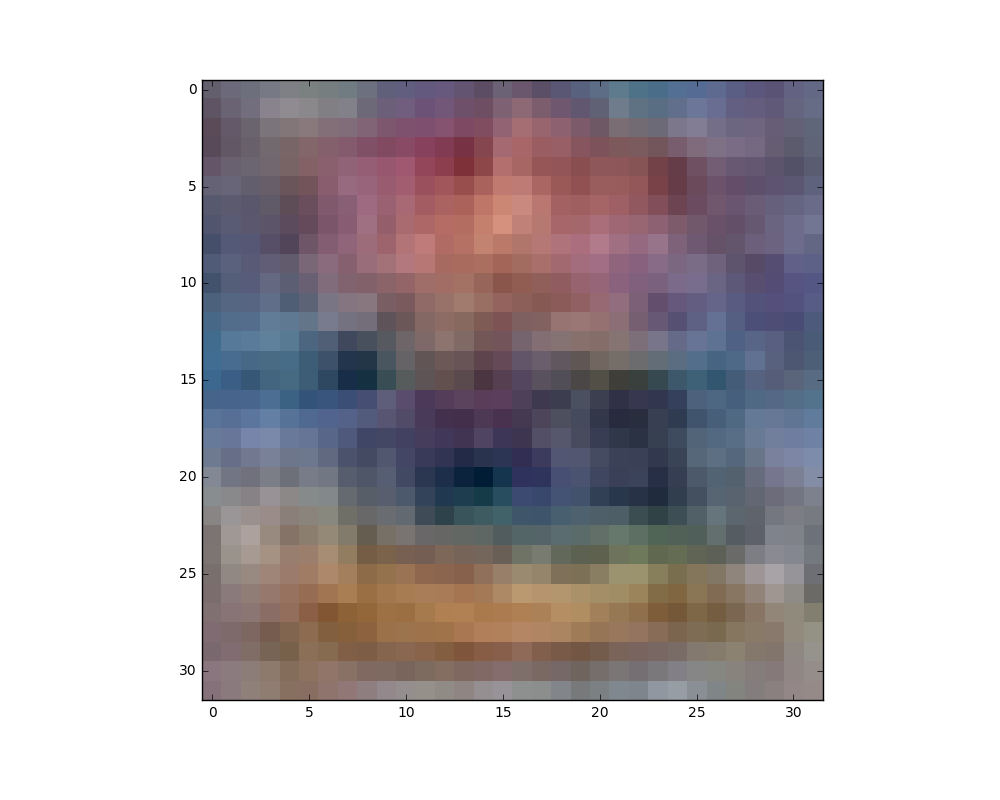
\includegraphics[height=1.25in, width=1.6in]{Figs4Paper/_final/svm_learnedweights_burger.eps}
        \caption{burger}
    \end{subfigure}
    \hskip2em
    \begin{subfigure}{.4\linewidth}
        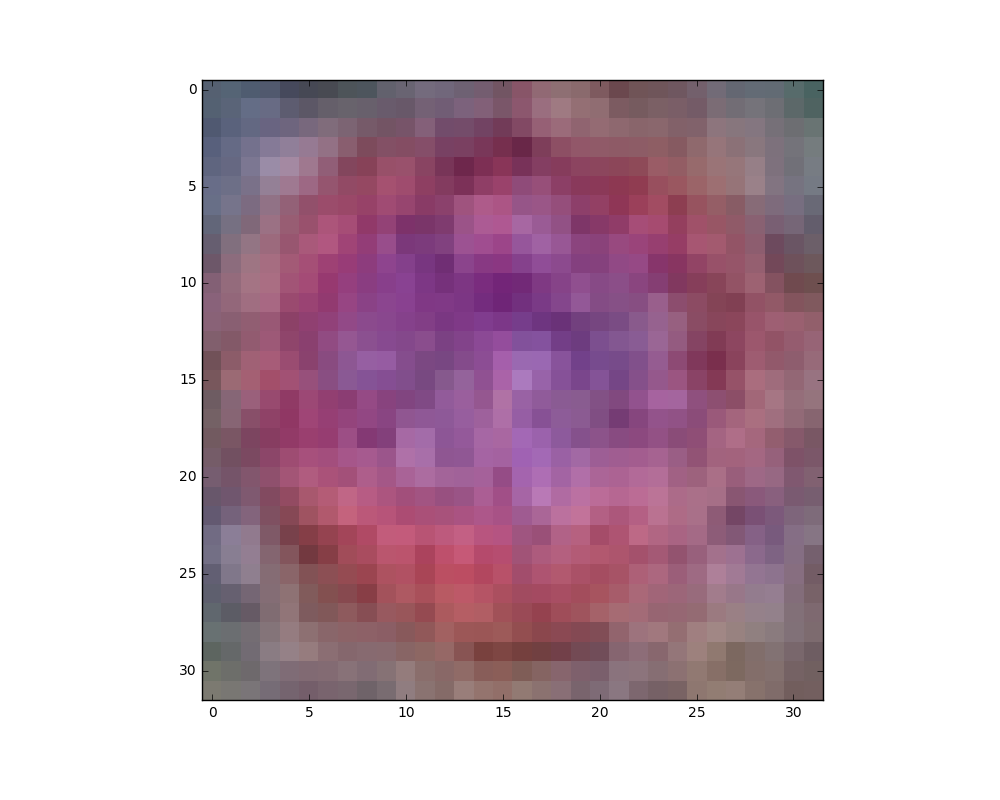
\includegraphics[height=1.25in, width=1.6in]{Figs4Paper/_final/svm_learnedweights_pizza.eps}
        \caption{pizza}
    \end{subfigure}
    \caption{Visualizing the weights learned by the SVM model}
		\label{fig:learnedweightsburgerpizza}
\end{figure}


To set our baseline, we first use a linear classifier using raw image pixels as features. For this we tried out both a SVM classifier and a Softmax classifier. The best validation accuracy of 0.18 was achieved using the SVM classifier with a learning rate 1e-07 and regularization strength 2.5e+04. The corresponding test set accuracy was 0.16.

One interpretation of a linear classifier is that of a \textit{template match}, where each row of the learned weights matrix corresponds to a template for the corresponding class. Figure~\ref{fig:learnedweightsburgerpizza} shows the learned weights for the burger and pizza classes in our dataset. We note that both the templates match our intuition; the burger contains a lot of brown pixels, the pizza has a round shape and contains a lot of red pixels at the center.   

\subsection{Neural networks on raw image pixels}
\label{subsec:neuralnetworksonrawimagepixels}

\begin{figure}[h!]
\centering
  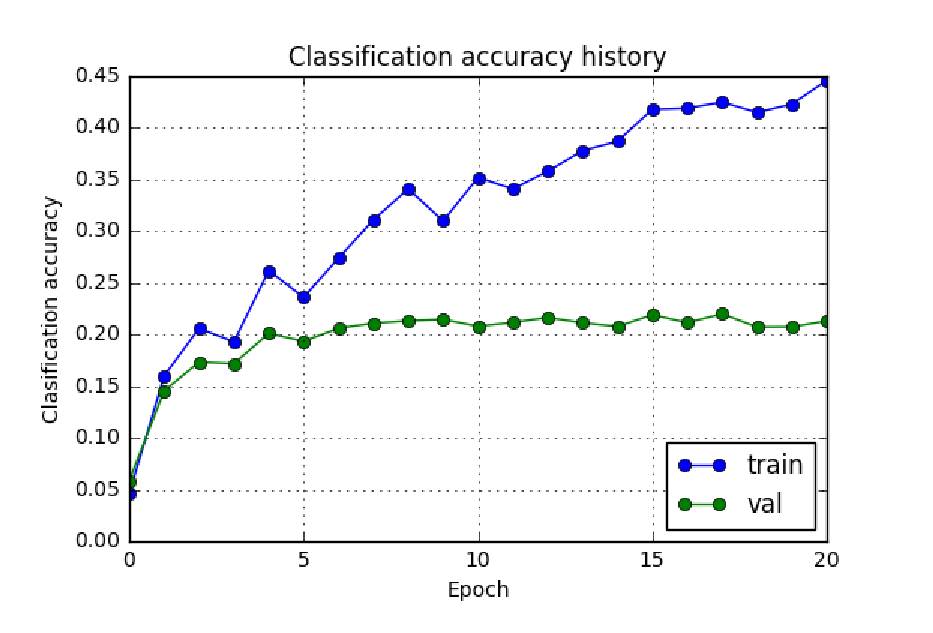
\epsfig{file=Figs4Paper/_final/fcfivelayer_rawpixels_classificationaccuracy.eps, height=1.5in, width=2.5in}
  \caption{Classification accuracy history of a fully connected five layer neural network using raw image pixels}
  \label{fig:fcfivelayerrawpixelsclassificationaccuracy}
\end{figure}

The next set of models we tried out were fully connected neural networks, again using raw image pixels as features.  Our network architecture was a six layer fully-connected network. Each of the five hidden layers had 100 neurons each. We used ReLU nonlinearity, and a softmax loss function. Below we note some interesting observations from training these models.

\begin{itemize}[noitemsep]
\item Batch normalization was~\cite{ioffe2015batch} \textbf{very useful} in training our model. Without batch normalization our model was performing quite poorly.
\item The best validation accuracy of 0.19 was achieved using the \textbf{Adam}~\cite{kingma2014adam} update rule with a learning rate of 1e-03. The test set accuracy was 0.18   
\end{itemize}

Figure~\ref{fig:fcfivelayerrawpixelsclassificationaccuracy} shows the classification loss history for the training and validation sets over 20 epochs while training this network.

\begin{figure*}[h!]
\centering
	\fbox{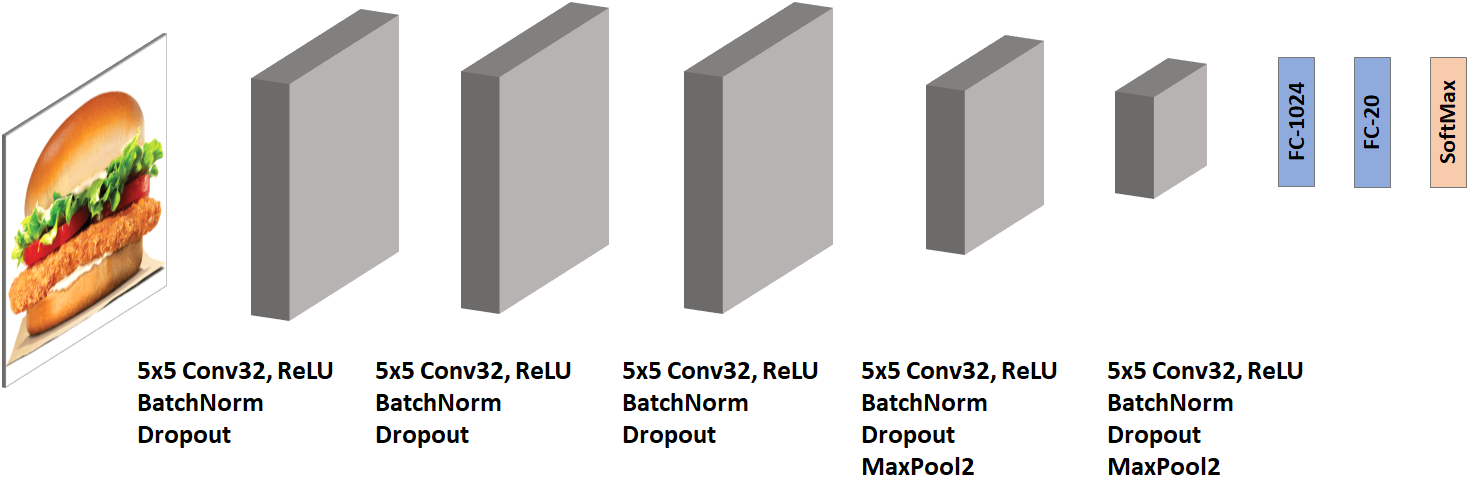
\includegraphics[width=12cm]{Figs4Paper/_final/convnet_architecture.eps}}
  \caption{Convolutional network architecture}
  \label{fig:convnetarchitecture}
\end{figure*}

\subsection{Image features}
\label{subsec:imagefeatures}


\begin{figure}[h!]
\centering
  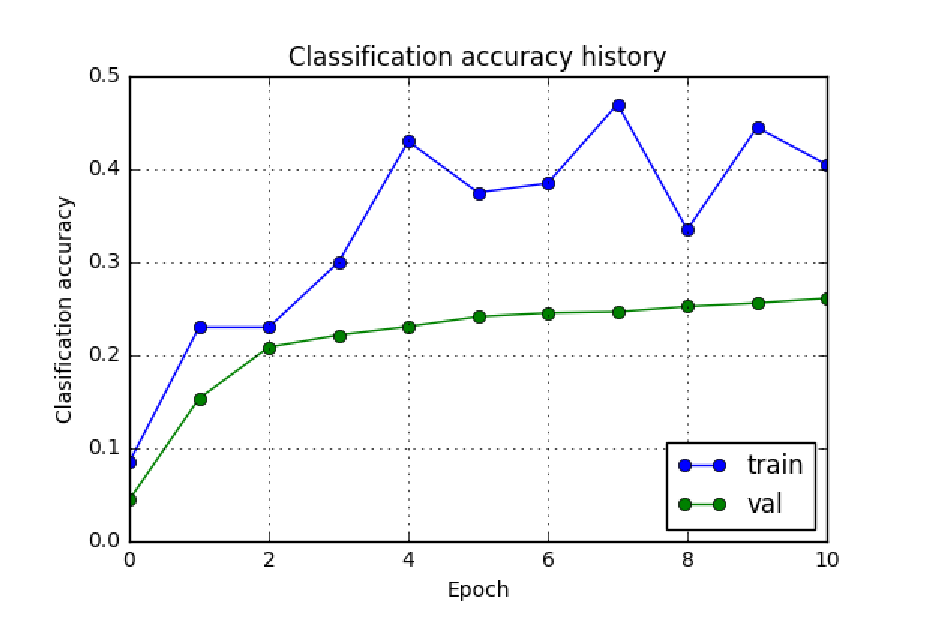
\epsfig{file=Figs4Paper/_final/imagefeatures_fctwolayer_classificationaccuracy.eps, height=1.5in, width=2.5in}
  \caption{Classification accuracy history of a fully connected two layer neural network using image features}
  \label{fig:imagefeaturesfctwolayerclassificationaccuracy}
\end{figure}

We did a set of experiments using features extracted from the images. For featurizing each image, we compute a Histogram of Oriented Gradients (HOG) as well as a color histogram using the hue channel in HSV color space. We form our final feature vector for each image by concatenating the HOG and color histogram feature vectors. This gives us a total of 155 features for each image. Below we summarize the results using image features with a SVM and a Two Layer Fully Connected Neural Network classifier.

\begin{itemize}[noitemsep]
\item Using the images features with a linear SVM classifier we were able to get a validation accuracy of 0.21, using SGD with a learning rate of 1e-03 and regularization strength of 1e+00
\item Using the images features with a Two Layer Fully Connected Neural Network gave much better performance. We got the best validation accuracy of 0.26 while using SGD as our update rule with a learning rate of 0.9, learning rate decay of 0.8 and regularization strength 0. The corresponding test set accuracy was 0.27   
\end{itemize}

Figure~\ref{fig:imagefeaturesfctwolayerclassificationaccuracy} shows the classification loss history for the training and validation sets over 10 epochs while training the Two Layer Fully Connected Neural Network classifier with image features.

\subsection{Convolutional Networks}
\label{subsec:convolutionalnetworks}

Using Convolutional Networks we were able to get the validation and test set accuracy of 0.40 each. Figure~\ref{fig:convnetarchitecture} shows the architecture we used. Below we note some of the things we tried out.

\begin{itemize}[noitemsep]
\item Batch normalization~\cite{ioffe2015batch} was quite useful in training our model.
\item For the weights in our network, using Xavier initialization~\cite{glorot2010understanding} helped.
\item Dropout~\cite{hinton2012improving, srivastava2014dropout} (with keep probability 0.75) helped improve the validation accuracy from 0.38 to 0.40. 
\item We kept the number of filters fixed at 32. 
\item We tried different sized filters (3x3, 5x5 and 7x7) but they did not help much. So we fixed the filter size at 5x5.
\item For the first three conv layers we preserve the height and width dimensions. For the fourth and fifth conv layers, we used max pooling with stride 2 (across both height and width).
\item After the five conv layers, we added two fully connected layers with 1024 and 20 neurons respectively. 
\item For the last layer we use softmax with cross entropy loss. 
\item The best validation accuracy of 0.40 was achieved using the \textbf{Adam}~\cite{kingma2014adam} update rule with a learning rate of 1e-04. The test set accuracy was 0.40. 
\end{itemize}

\begin{figure}[h!]
\centering
  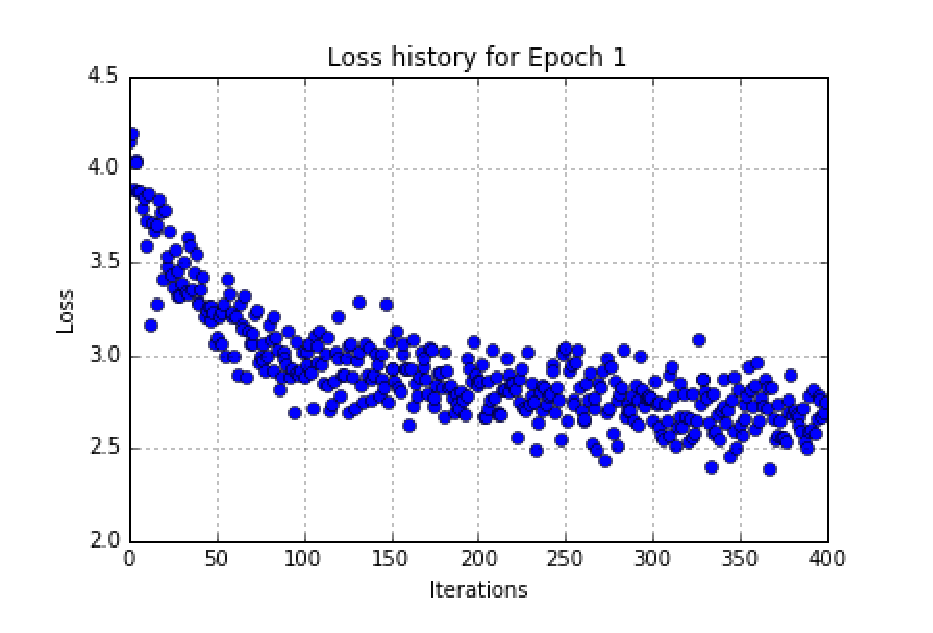
\epsfig{file=Figs4Paper/_final/convnet_losshist_epoch1.eps, height=1.5in, width=2.5in}
  \caption{Reduction in loss over several mini-batches in the first epoch of the convolutional network}
  \label{fig:lossepoch1}
\end{figure}

Figure~\ref{fig:lossepoch1} shows the reduction in the loss over multiple iterations in the first epoch. We see the loss reduces very sharply in the beginning, and then flattens out gradually.  

\begin{figure}[h!]
\centering
  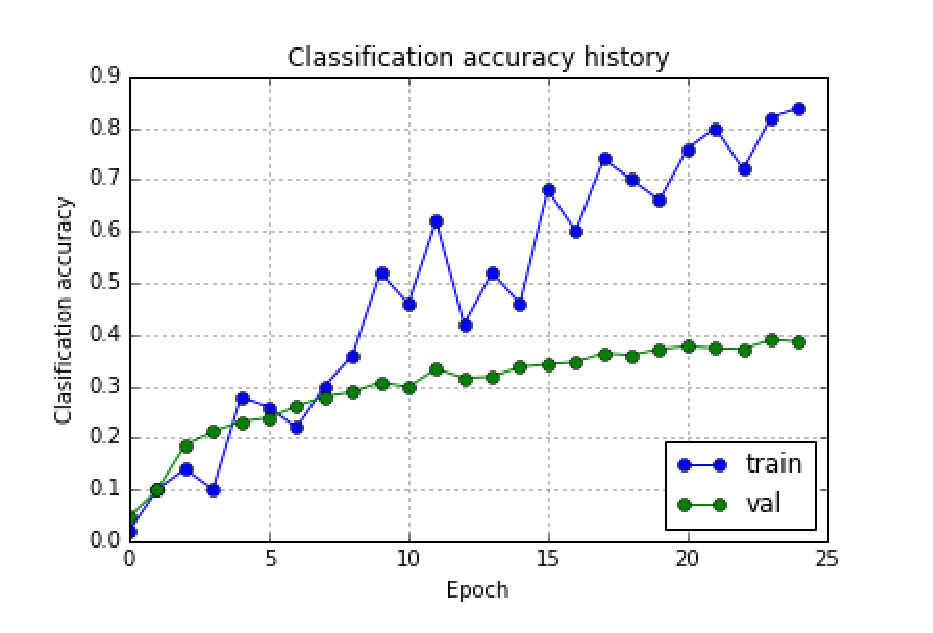
\epsfig{file=Figs4Paper/_final/convnet_classificationaccuracy.eps, height=1.5in, width=2.5in}
  \caption{Classification accuracy history of the convolutional network over 25 epochs}
  \label{fig:convnetclassificationaccuracy}
\end{figure}

Figure~\ref{fig:convnetclassificationaccuracy} shows the classification loss history for the training and validation sets over 25 epochs of the conv net.

\subsection{Transfer Learning}
\label{subsec:transferlearning}

\begin{figure}[h!]
\centering
  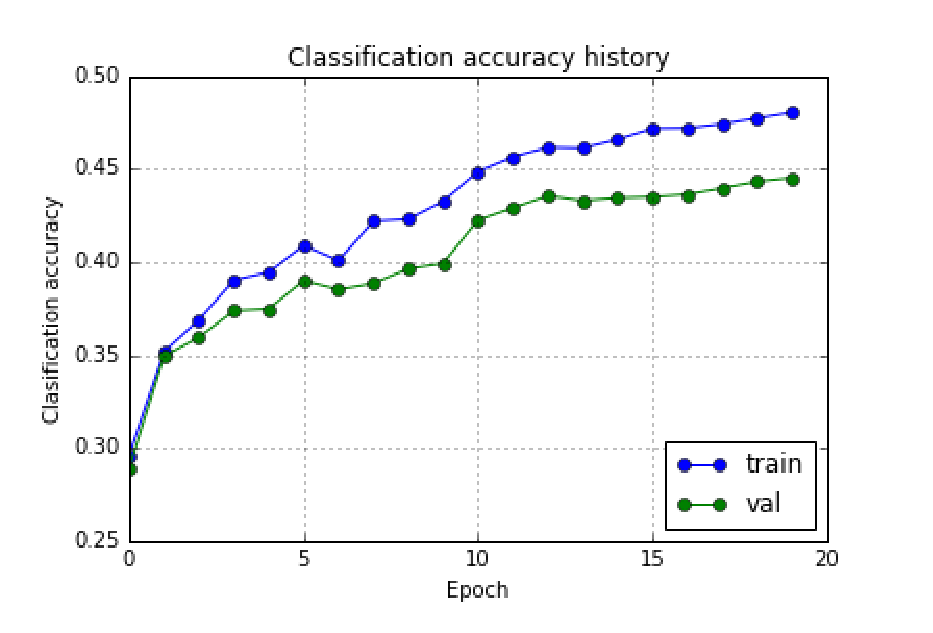
\epsfig{file=Figs4Paper/_final/transferlearning.eps, height=1.5in, width=2.5in}
  \caption{Classification accuracy history after fine-tuning a VGG model}
  \label{fig:transferlearning}
\end{figure}

To improve the accuracy of our model further, we did a set of experiments around transfer learning. Interestingly this gave us the best results on our dataset.  Some salient observations from this approach are as follows:

\begin{itemize}[noitemsep]
\item We are using the VGG-16~\cite{simonyan2014very} model pretrained on ImageNet
\item We remove the last fully connected layer (fc8) and replace it with our own, with output size 20
\item We first train the last layer for 10 epochs. This allows us to get meaningful weights for the fc8 layer first.  Subsequently, we train the entire model on our dataset for 10 more epochs.
\end{itemize}

For this approach, we referenced the TensorFlow finetune sample on GitHubGist~\cite{finetunegithubgist}. Following the example in the gist, we did similar pre-processing on our dataset to make it work for the VGG-16 model. The pre-processing steps are listed below:

\begin{itemize}[noitemsep]
\item Resize the image so its smaller side is 256 pixels long. Recall that our existing dataset has dimensions (32, 32, 3).
\item Take a random 224x224 crop of the scaled image (for the train, validation and test sets)
\item Horizontally flip the image with probability 1/2 (for the train set only)
\item Substract the per color mean VGG\_MEAN [123.68, 116.78, 103.94) (for the train, validation and test sets)
\end{itemize}


Figure~\ref{fig:transferlearning} shows the classification loss history for the training and validation sets over all the 20 epochs. Table~\ref{table:accuracyresults} shows a summary of results across different modeling approaches.





\section{Conclusion}
\label{sec:conclusion}

We observe that convolutional neural networks are quite suitable for the task of classifying food dishes, and outperform traditional machine learning approaches at this task. The transfer learning approach looks most promising, especially because both the training and validation accuracy are improving with the number of epochs (i.e. we have not overfit our model). This suggests that more data (and/or running it for more epochs) could improve the accuracy metric further. 

From a  data collection perspective, we plan on leveraging ImageNet~\cite{imagenet} and Flickr~\cite{flickr} to build a larger dataset of images. From a modeling perspective, we also want to try out using convolutional nets as a \textit{fixed feature extractor}, and use the extracted features with linear classifiers or decision trees to improve accuracy. 

There are several interesting problems around food images that we wish to investigate in the future. This includes being able to detect individual food items on plate, accurately predicting the number of calories given an image of a food dish etc. Convolutional networks seem to be a natural fit for these visual recognition tasks.  


%------------------------------------------------------------------------
{\small
\bibliographystyle{ieee}
\bibliography{egbib}
}

\end{document}
